\documentclass[a4paper]{article}

\usepackage{reportFormat}


\title{
	\Large {\sc Mech}4450 Aerospace Propulsion \\
	\Huge Major Assignment - Part 2
}

\author{
	Muirhead, Alex \\ \texttt{s4435062}
	\and
	Watt, Robert \\ \texttt{s4431151}
}

\date{\today}



\begin{document}

\pagenumbering{gobble}
\maketitle

\vfill

\begin{abstract}
    The proposed \textsc{Spartan} scramjet engine is analysed to determine the feasibility of using ethylene as the fuel. The operation of the engine at a free stream Mach number of 10 is studied. The inlet was modelled using high resolution computational fluid dynamics, the combustor was modelled using a finite rate chemistry model, and the nozzle was modelled as an isentropic expansion with a velocity factor applied to account for losses. Each engine was found to be capable of producing 14.5~kN of positive thrust. With four engines in each \textsc{Spartan} vehicle can produce 29~kN of net force, accounting for drag, with a thrust margin of 1.01. The specific thrust of each engine is \SI{468.32}{\N \s \per \kg}, and the specific impulse of each engine is \SI{47.74}{\s}. However the maximum temperature within the combustion was approximately 3500~K, so further investigation into the wall temperature is required to make sure that the wall materials can support the thermal load. Finally, further investigation into the performance of the engines at lower Mach numbers is required to ensure the engine is capable of reaching speeds of Mach 10. This investigation hasn't ruled out the possibility of using a ethylene fuelled engine for the \textsc{Spartan} second stage vehicle, however further research is needed to ensure the feasibility. 
\end{abstract}

% \tableofcontents

\vspace{10em}

\newpage

\tableofcontents
\pagenumbering{roman}
\newpage
\section*{Nomenclature}

\begin{table}[H]
    \centering
    \begin{tabu} spread 0cm {X[-1,c]X[-1,l]X[-1, r]}
        \toprule \rowfont[c]{\bfseries}
             Symbol     &                     Usage                    &        Standard unit        \\ 
        \midrule
        \(M\)           & Mach number                                  & -                           \\
        \(x\)           & Position along combustion chamber            & \si{\m}                     \\
        \(\gamma\)      & Ratio of specific heats                      & -                           \\
        \(R\)           & Specific gas constant                        & \(\si{\J\per\kg\per\K}\)    \\
        \(A\)           & Combustor cross sectional area               & \(\si{\m \squared}\)        \\
        \(T\)           & Static temperature                           & \(\si{\K}\)                 \\
        \(T_t\)         & Stagnation temperature                       & \(\si{\K}\)                 \\
        \(C_f\)         & Skin friction coefficient of combustor walls & -                           \\
        \(D\)           & Local diameter of combustor                  & \(\si{\m}\)                 \\
        \(c_{p}\)       & Specific heat at constant pressure           & \(\si{\J \per \g \per \K}\) \\
        \(Y\)           & Species mass fraction                        & -                           \\
        \([X]\)         & Species concentration                        & \(\si{\kmol\per\m\cubed}\)  \\
        \(h_{f}^\circ\) & Enthalpy of formation                        & \(\si{\kJ\per\kmol}\)       \\
        \(\mathcal{M}\) & Species molecular weight                     & \(\si{\kg\per\kmol}\)       \\
        \(v\)           & Local flow velocity                          & \(\si{\m\per\s}\)           \\
        \(\rho\)        & Density                                      & \(\si{\kg\m\cubed}\)        \\
        \(P\)           & Static pressure                              & \(\si{\Pa}\)                \\
        \(q\)           & Dynamic pressure                             & \(\si{\kPa}\)               \\
        \(F\)           & Thrust                                       & \si{\N}\\
        SF & Specific thrust & \si{\N \s \per \kg}\\
        \(I_{s}\)            & Specific impulse                        & \si{\s}\\
        \bottomrule 
    \end{tabu}
    \caption{Nomenclature}
    %\label{tab:freestream values}
\end{table}

\begin{table}[H]
    \centering
    \begin{tabu} spread 0cm {X[-1,r]X[-1,c]}
        \toprule \rowfont[c]{\bfseries}
              Subscript & usage\\ \midrule
              0 & free stream state\\
              3 & combustor inlet state\\
              4 & combustor outlet state\\
              10 & nozzle exit state\\
              \(i\) & an individual species \\
              \(b\) & burner, used for fuel-air mixtures\\
        \bottomrule 
    \end{tabu}
    \caption{Subscripts}
    %\label{tab:freestream values}
\end{table}

\newpage
\pagenumbering{arabic}

\section{Introduction}
The University of Queensland and our partners are developing a 3-stage, 93\% reusable, partially air-breathing small satellite launch system known as \textsc{Spartan} (Scramjet Powered Accelerator for Reusable Technology AdvaNcement). The \textsc{Spartan} mission profile is shown in Fig.~\ref{fig:mission_profile}. A rocket powered \nth{1} stage accelerates the vehicle stack to the minimum operating Mach number of the scramjet powered second stage (Mach 5). The \nth{1} stage is then jettisoned and returns to base, and the scramjet accelerates the remainder of the vehicle to the scramjet cut-off Mach number of 10. A rocket powered \nth{3} stage then separates from the second stage and accelerates the payload to orbit, while the second stage flies back to base.

\begin{figure}[H]
    \centering
    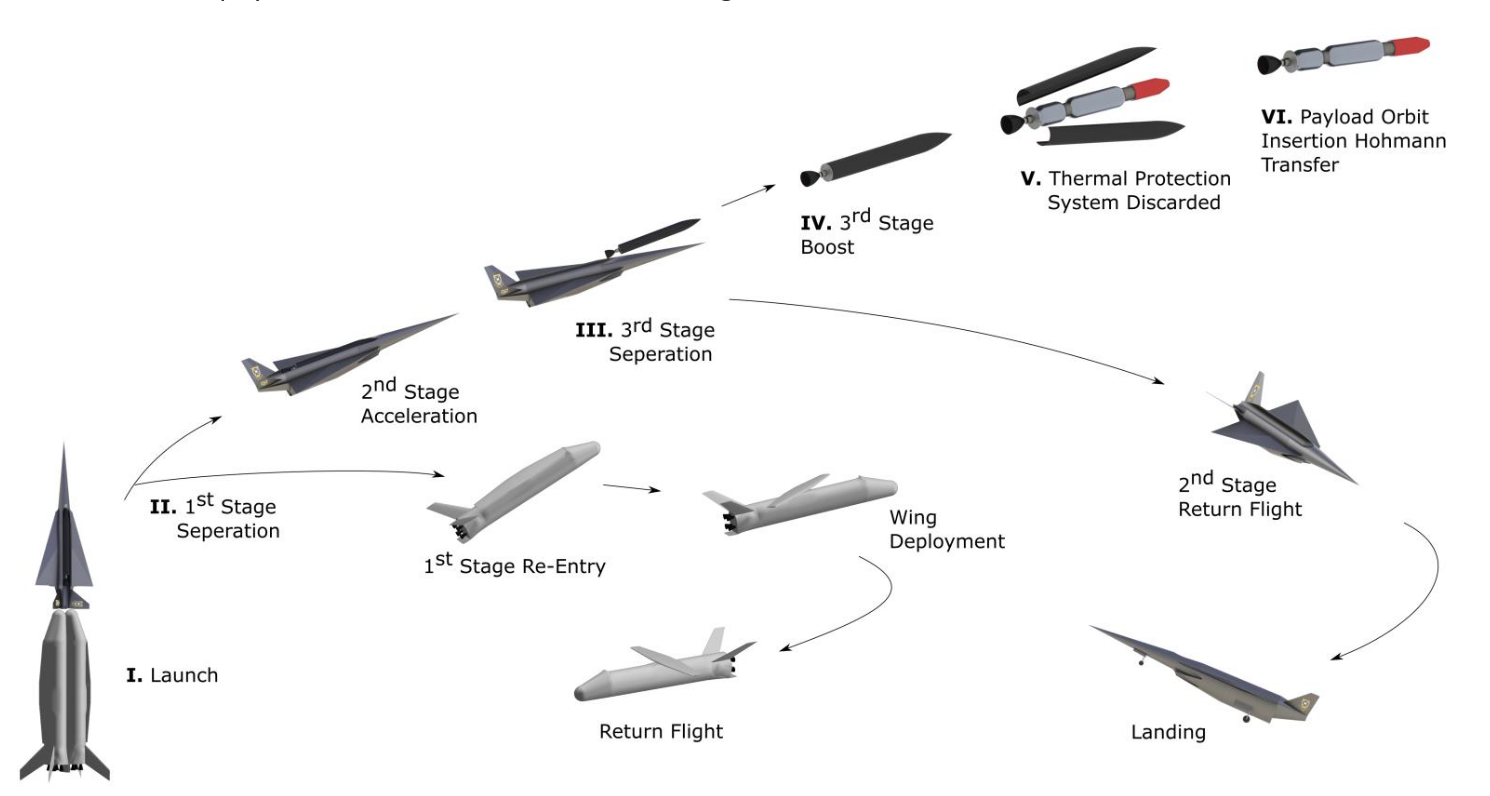
\includegraphics[width=0.9\linewidth]{part_2_img/spartan_overview.png}
    \caption{\textsc{SPARTAN} mission profile}
    \label{fig:mission_profile}
\end{figure}

The present \textsc{Spartan} design requires the second stage be fuelled with liquid hydrogen, since it is the most energetic fuel and gives the best propulsive performance. Even in its liquid form, however, hydrogen has low density and it is marginal whether the fuel tanks and required flight systems can be successfully packaged within the vehicle (this means it is possible, but even a small change in e. g. required wall thickness could cause the available volume to be insufficient). Furthermore, liquid hydrogen infrastructure is available at only a small subset of potential launch sites, which would greatly restrict where \textsc{Spartan} could be deployed. Both of these issues would be overcome if it was possible to fuel the scramjet with a denser hydrocarbon fuel, but this is challenging at high Mach numbers as hydrocarbon fuels have longer ignition and reaction times, and are less energetic. For this reason, the most promising hydrocarbon fuel for \textsc{Spartan} is ethylene (\(\ce{C2H4}\)) as it is the fastest reacting. UQ has had recent successes in experiments of supersonic combustion of ethylene in scramjet at Mach 8 [1, 2], but it is unknown if net thrust can be generated using ethylene fuel at Mach 10, where the time available for ignition and combustion is least. We would like you to be the engineering consultants who investigate this issue.

\section{Project Brief}
The task is to assess if the thrust generated by the scramjet powered second stage of the \textsc{Spartan} can exceed vehicle drag during Mach 10 flight (M = 10) if ethylene fuel is used. Whether the flow residence time within the engine is sufficiently long for reactions to proceed to completion is a key consideration, thus you modelling must incorporate the effects of finite rate chemistry. Part 1 of this project will focus on developing a chemistry module that takes the current temperature and pressure of the gas mixture as an input, internally computes the reaction rates and updates the mixture composition, the outputs the rate of heat released to the combustor. In Part 2 this module will be used within a quasi-one-dimensional cycle analysis to compute the performance of the scramjet.

\section{Methodology}\label{sec:methodology}

\subsection{Combustor modelling}
Combustion was modelled using the same model that was developed in part 1, however the temperature was calculated at each step along the solution from the heat released during combustion, rather than assuming a temperature profile ahead of time.

In order to calculate the temperature needed by the chemistry model, and also to calculate thrust, the total temperature and Mach number must be solved alongside the chemistry model. The additional equations to be solved are Eq.~\ref{eqn:dM2dx} and \ref{eqn:dTtdx}. Note that even though \(\ce{N2}\) doesn't react, it is included in the differential equations to be solved. Thus sums over reacting species become sums over all species, and scaling of reacting species' mass fractions to the mass fraction of \(\ce{N2}\) isn't needed.
\begin{align}\label{eqn:dM2dx}
    \frac{\partial M^2}{\partial x} =M^2 \frac{1 + \frac{\gamma_b - 1}{2}M^2}{1-M^2}\left( -\frac{2}{A} \frac{\partial A}{\partial x} + \frac{1 + \gamma_b M^2}{T_t}\frac{\partial T_t}{\partial x} + \frac{4 \gamma_b M^2 C_f}{D}\right)
\end{align}
\begin{align}\label{eqn:dTtdx}
    \frac{\partial T_t}{\partial x} = - \frac{1}{c_{pb}}\sum_i \frac{\partial Y_i}{\partial x}h_{f,i}^\circ
\end{align}
Where the gradients of mass fraction and concentration for individual species are given in Eq.~\ref{eqn:spatial_mass_fraction_gradient} and~\ref{eqn:spatial_concentratoin_gradient}.
\begin{gather}
    \label{eqn:spatial_mass_fraction_gradient}
    \frac{\partial Y_i}{\partial x} = \mathcal{M}_i \left\lbrace \frac{1}{\sum_j \left[X_j\right]\mathcal{M}_j} \frac{\partial \left[X_i\right]}{\partial x} - \frac{\left[ X_i \right]}{\left(\sum_j \left[X_j\right]\mathcal{M}_j \right)^2 }\sum_j \mathcal{M}_j\frac{\partial \left[ X_j \right]}{\partial x} \right\rbrace \\
    \label{eqn:spatial_concentratoin_gradient}
    \frac{\partial \left[X_j\right]}{\partial x} = \frac{1}{v}\frac{\partial \left[X_j\right]}{\partial t}
\end{gather}
The modelling of the rate of concentration change in given in Sec.~\ref{subsec:finite rate chem}. This rate is divided by the local gas velocity \(v\), which converts the time derivatives computed by the chemistry model into spatial derivatives needed to model the combustion. The velocity can be found using the local Mach number of the flow.
\begin{align}\label{eqn:v(x)}
    v = M \sqrt{\gamma_b R_b T}
\end{align}
Since \(T_t\) and \(M\) are solved for at each time step, \(T\) can be calculated using isentropic flow relations (Eq.~\ref{eqn:T(x)}). This is needed by the chemistry model, and to calculate \(v\).
\begin{equation}\label{eqn:T(x)}
    T = T_t \left[ 1 + \frac{\gamma_b-1}{2}M^2 \right]^{-1}
\end{equation}
The cross-sectional area of the combustor is a linear function of the length-wise position and initial combustor area, and is given along with the respective area gradient in Eq.~\ref{eqn:area} and~\ref{eqn:area grad}
\begin{gather} 
    \label{eqn:area}
    A(x) = A_3 \frac{1 + 3x}{L} \\
    \label{eqn:area grad}
    \frac{\partial A}{\partial x} = \frac{3A_3}{L}
\end{gather}
Thus, using all the above equations, a system of ordinary differential equations can be solved to give the mass fraction of each species, total temperature and Mach number at each point along the combustor.
\begin{align}
    \frac{\partial}{\partial x} 
    \begin{bmatrix}
    \left[ X \right] \\
    T_t\\
    M^2
    \end{bmatrix}
    =
    \begin{bmatrix}
        f_0 \left(T_t, M^2, \left[ X \right]\right)\\
        f_1 \left(T_t, M^2, \left[ X \right]\right)\\
        f_2 \left(T_t, M^2, \left[ X \right]\right)
    \end{bmatrix}
\end{align}
Additionally, the density of the flow at each point along the combustor can be calculated from conservation of mass.
\begin{align}
    \rho = \frac{\dot{m}}{v A(x)}
\end{align}
This density can then be used to calculate the pressure at each point in the combustor using the ideal gas law.
\begin{align}
    P = \rho R T
\end{align}

\subsection{Finite Rate Chemistry}\label{subsec:finite rate chem}
For a given chemical reaction \(j\) containing species \(X\), that can be expressed in the form 
\begin{equation}
    \sum_i \nu_{f,i} X_i \ce{->} \sum_i \nu_{b,i} X_i 
\end{equation}
the rate of change of concentration due to this reaction for any given species is approximated by
\begin{equation}\label{eqn:rate of reaction}
    \left(\frac{d [X_i]}{d t} \right)_j
    = (\nu_{b,i}-\nu_{f,i}) \left\lbrace k_f \prod_k [X_k]^{\alpha_k} - k_r \prod_k [X_k]^{\beta_k} \right\rbrace
\end{equation}
where \(\alpha\) and \(\beta\) are experimentally determined exponents in the case of non-elementary reactions, and are equal to \(\nu_f\) and \(\nu_b\) for elementary reactions. The total rate of change of concentration for a species \(X_i\) is then given by the contributions of all reactions. 
\begin{equation}
    \frac{d [X_i]}{d t} = \sum_j \left(\frac{d [X_i]}{d t} \right)_j
\end{equation}
The forward reaction rate coefficient \(k_f\) from Eq.~\ref{eqn:rate of reaction} is calculated through the Arrhenius equation (Eq.~\ref{eqn:arrhenius}), while the backward reaction rate coefficient \(k_b\) is governed by the equilibrium constant \(K_c\).
\begin{gather}
    \label{eqn:arrhenius}
    k_f = A\exp\left(\frac{-E_a}{R_uT}\right) \\
    k_b = \frac{k_f}{K_c}
\end{gather}
Constant values for the pre-exponential factor \(A\) and activation energy \(E_a\) are specific to each reaction, and are well documented.  The equilibrium constant may be calculated by relation to the product of the pressure constants of each species (Eq.~\ref{eqn:equilibrium constant}), which themselves are related to the respective Gibbs free energy values (Eq.~\ref{eqn:pressure constant}). 
\begin{gather}
    \label{eqn:equilibrium constant}
    K_c = \prod_i K_{p,i} \left(\frac{P^\circ}{R_u T}\right)^{(\beta_i-\alpha_i)} \\
    \label{eqn:pressure constant}
    K_{p,i} = \exp\left(\frac{-\Delta G^\circ_{f,i}}{R_u T}\right)
\end{gather}
It should be noted that the Gibbs free energy (\(\Delta G^\circ_{f,i}\)) is dependent on temperature, however values are tabulated for common chemical species over large ranges of temperatures. 

\subsection{Nozzle Modelling}\label{subsec:nozzle_modelling}
The flow within the nozzle is assumed to isentropically expand from the combustor exit pressure to \(3P_0\). Losses within the nozzle are then quantified by assuming a velocity coefficient of 0.95. Using isentropic flow relations, it can be shown that the Mach number of the exhaust is given by Eq.~\ref{eqn:exhaust_mach}. Note that primed states refer to the ideal exhaust state, before nozzle losses have been accounted for.

\begin{align}\label{eqn:exhaust_mach}
    M_{10}^\prime = \sqrt{\frac{2}{\gamma_b - 1} \left[ \left(\frac{P_4}{P_{10}} \right)^{\frac{\gamma_b-1}{\gamma_b}}\left( 1 + \frac{\gamma_b - 1}{2}M_4^2 \right) - 1 \right]}
\end{align}
The ideal exhaust temperature can then be calculated assuming isentropic expansion from state 4 to state 10'.
\begin{align}\label{eqn:T10_dash}
    T_{10^\prime} = T_4 \frac{2 + (\gamma_b - 1) M_4^2}{2 + (\gamma_b - 1) M_{10}^{\prime 2}}
\end{align}

Using Eq.~\ref{eqn:T10_dash} and \ref{eqn:exhaust_mach}, the ideal exhaust velocity can be determined by rearranging the definition of Mach number. The velocity factor can then be applied to compensate for the non ideal behaviour of the nozzle.
\begin{equation}\label{eqn:v10_dash}
    v_{10} = 0.95 M_{10}^\prime \sqrt{\gamma_b R_b T_{10}^\prime}
\end{equation}
With the actual exhaust velocity known, the actual exhaust temperature and Mach number can be calculated using conservation of energy and the definition of Mach number.
\begin{align}
    T_{10} &= T_{t4} - \frac{v_{10}^2}{2c_{pb}} \label{eqn:T10} \\
    M_{10} &= \frac{v_{10}}{\sqrt{\gamma_b R_b T_{10}}} \label{eqn:M10}
\end{align}
The density of the exhaust can calculated using the ideal gas law applied to the nozzle exit.
\begin{equation}
    \rho_{10} = \frac{P_{10}}{R_b  T_{10}}
\end{equation}
And finally, the area of the nozzle exit can be calculated using conservation of mass.
\begin{equation}
    A_{10} = \frac{\dot{m}}{\rho_{10}v_{10}}
\end{equation}
\subsection{Performance Parameters}
It can be shown, using a momentum balance of the air moving through the engine, that the thrust of each engine is
\begin{equation}\label{eqn:thrust}
    F = \dot{m}\left( v_{10} - v_0 \right) + A_{10}\left( p_{10} -  p_0 \right)
\end{equation}
The specific thrust is defined as the thrust per unit mass of fuel through the engine
\begin{equation}
    ST = \frac{F}{\dot{m}}
\end{equation}
And the specific impulse is the specific thrust normalised by the acceleration due to gravity at sea level on Earth.
\begin{equation}
    I_{sp} = \frac{F}{g_0 \dot{m}}
\end{equation}
And finally, the thrust margin is defined as
\begin{equation}
    \mathrm{Thrust \, margin} = \frac{thrust - drag}{drag}
\end{equation}

\newpage
\section{Results and Discussion}
\subsection{Inlet Modelling}
The flight conditions of the scramjet can be used to calculate properties of the gas entering the scramjet. Given values for the freestream flight conditions are listed in Table.~\ref{tab:freestream values}. 
\begin{table}[H]
    \centering
    \begin{tabu} spread 0cm {X[-1,l]X[-1,c]X[-1,r]}
        \toprule \rowfont[c]{\bfseries}
               Property       &  Symbol &           Value           \\
        \midrule 
                  Mach Number & \(M_0\) &                        10 \\
           Static Temperature & \(T_0\) &              \SI{220}{\K} \\
             Dynamic Pressure & \(q_0\) &             \SI{50}{\kPa} \\
        Specific Gas Constant &  \(R\)  & \SI{287}{\J\per\kg\per\K} \\
        \bottomrule 
    \end{tabu}
    \caption{Freestream flight conditions}
    \label{tab:freestream values}
\end{table}
Using the static temperature to calculate the speed of sound \(a_0^2 = \gamma R T_0\), and the flight Mach number, the velocity of gas entering the scramjet is given as:
\begin{equation}
    v_0 = M_0 \sqrt{\gamma R T_0} = \SI{2973}{\m\per\s}
\end{equation}
The vehicle operates at constant dynamic pressure, given by the relation \(q_0 = \frac{1}{2}\rho_0v_0^2\). With velocity known, this can be rearranged to give the inlet density, and subsequently pressure from the ideal gas law. 
\begin{gather}
    \rho_0 = \frac{2 q_0}{v_0^2} = \SI{0.011}{\kg\per\m\cubed} \\
    p_0 = \rho_0 R T = \SI{714.4}{\Pa}
\end{gather}
The capture area of the inlet can be calculated knowing the mass flow rate of air into the scramjet (found in Sec.~\ref{sec:Combuster Modelling}) and the specific properties above. 
\begin{equation}
    A_0 = \frac{\dot{m}_\text{air}}{\rho_0 v_0} = \SI{0.87}{\m\squared}
\end{equation}

\subsection{Combustor Modelling}
\label{sec:Combuster Modelling}
As the fuel is mixed with the incoming airflow, the specific properties of the gas change due to the composition change and compression through oblique shocks. Properties at the start of the combustor were determined through CFD modelling of the inlet, and assumes that all fuel is perfectly mixed. 
\begin{table}[H]
    \centering
    \begin{tabu} spread 0cm {X[-1,l]X[-1,c]X[-1,r]}
        \toprule \rowfont[c]{\bfseries}
                 Property       &      Symbol     &             Value             \\
        \midrule 
                    Mach Number & \(M_{3b}\)     &                         3.814 \\
             Static Temperature & \(T_{3b}\)     &              \SI{1237.63}{\K} \\
                Static Pressure & \(p_{3b}\)     &              \SI{70.09}{\kPa} \\
          Specific Gas Constant & \(R_{b}\)      & \SI{288.450}{\J\per\kg\per\K} \\
        Ratio of Specific Heats & \(\gamma_{b}\) &                        1.3205 \\
           Mixed Mass Flow Rate & \(\dot{m}\)    &         \SI{31.12}{\kg\per\s} \\
        \bottomrule 
    \end{tabu}
    \caption{Combustor inlet gas properties}
    \label{tab:combuster inlet}
\end{table}
\vspace{-1em}
Using the ratio of specific heats and gas constant determined from the CFD modelling of the inlet, the specific heat at constant pressure for the air fuel mixture can be calculated. 
\begin{equation}
    c_{pb} = \frac{\gamma_b}{\gamma_b - 1}R_b = \SI{1.18845}{\kJ\per\kg\per\K}
\end{equation}
Assuming the ideal gas low still holds, the density of the air fuel mixture at the inlet to the combustor can be determined from the known static pressure and temperature.
\begin{equation}
    \rho_{3b} = \frac{P_{3b}}{RT_{3b}} = \SI{0.174}{\kg\per\m\cubed}
\end{equation}
The fuel is injected in a stoichiometric ratio, which can be determined from the global reaction of \ce{C2H4} and air. Assuming a standard molar ratio of 1:3.76 for \ce{O2}:\ce{N2}, this gives the following fuel-to-air ratio, which can then be used to calculate the initial mass flow of air captured by the scramjet inlet.  
\begin{gather}
    \ce{C2H4 + 3(O2 + 3.76N2) -> 3CO2 + 2H2O} \\
    \phi = 1 \quad \rightarrow 
    \quad f = \frac{m_\text{fuel}}{m_\text{air}} 
    = \frac{
        n_{\ce{C2H4}} \mathcal{M}_{\ce{C2H4}}
    }{
        n_{\ce{O2}} \mathcal{M}_{\ce{O2}} + 3.76 n_{\ce{N2}} \mathcal{M}_{\ce{N2}}
    }
    \approx \num{6.81e-2} \\
    \dot{m}_\text{air} = \frac{\dot{m}}{1 + f} \approx \SI{29.13}{\kg\per\s}
\end{gather}
The area of the inlet to the combustor, \(A_3\), can be calculated from conservation of mass applied to the fully mixed air-fuel mixture at the combustor inlet.
\begin{equation}
    A_3 = \frac{\dot{m}}{\rho_{3b} v_{3b}} = \SI{0.06}{\m\squared}
\end{equation}
The stagnation temperature of the flow into the combustor can be calculated using the known Mach number of flow at state 3.
\begin{equation}
    T_{t3} = T_{3b} \left(1 +\frac{\gamma_b - 1 }{2}M_{3b}^2\right) = \SI{4122.7}{\K}
\end{equation}
The velocity of the flow entering the combustor can be calculated from the Mach number of temperature as follows
\begin{equation}
    v_{3b} = M_{3b} \sqrt{\gamma_b R_b T_{3b}} = \SI{2618}{\m\per\s}
\end{equation}
And the density of the flow entering the combustor can be calculated using the ideal as law.
\begin{equation}
    \rho_{3b} = \frac{p_{3b}}{R_b R_{3b}} = \SI{0.196}{\kg\per\m\cubed}
\end{equation}
To progress the flow along the combustor, the system of equations presented in Section~\ref{sec:methodology} was solved using python (script provided in Appendix~\ref{app:code}). The engine performance at three different inflow temperatures (\SIlist{1000;1237.63;1400}{\K} ) were calculated. Plots of properties for each of these inflow temperatures along the combustor are plotted in Figs.~\ref{fig:properties_1000}, \ref{fig:properties_1238}, and \ref{fig:properties_1400} respectively. As can be seen, ignition doesn't occur at either \SI{1000}{\K} or \SI{1237.63}{\K}, however it does occur at \SI{1400}{\K}. The fraction of fuel burned for each inflow temperature is summarised in Table.~\ref{tab:fuel_burned}.
\begin{table}[H]
    \centering
    \begin{tabu} spread 0cm {X[-3,c]*{3}{X[-1,c]}}
        \toprule
        Inflow Temperature (\(T_{3b}\)) & \SI{1000}{\K} & \SI{1237.63}{\K} & \SI{1400}{\K} \\
        Mass fraction of fuel burned &  0.00028 & 0.01099 & 1.00000 \\
        \bottomrule
    \end{tabu}
    \caption{Mass fraction of fuel burned for test cases}
    \label{tab:fuel_burned}
\end{table}
As can be seen, the mass fraction of fuel burned increases as the temperature rises, as expected. Once the fuel ignites, all of the fuel in burned.

The plot of stagnation temperature in Fig.~\ref{fig:properties_1400} is particularly useful to see when ignition occurs (when the temperature reaches \(1.15 T_{t3}\), indicated on the graph). By determining when the stagnation temperature reaches the ignition temperature, it was possible to determine that ignition began 0.137~m along the combustor. Additionally, the point where the fuel runs out is evident in the sharp corner in the plot. The fuel runs out 0.142~m along the combustor. Thus the distance between ignition and burn out is 0.005~m, or 5~mm. The fuel burns extremely quickly once it ignites.

The state of the flow at the exit of the combustor is summarised in Table.~\ref{tab:combustor_exit_properties}.

\begin{table}[H]
    \centering
    \begin{tabu} spread 0cm {X[-1,c]X[-1,c]}
        \toprule \rowfont[c]{\bfseries}
            Variable      &      Value       \\
        \midrule
              Mach Number &             2.82 \\
              Temperature & \SI{2925.27}{\K} \\
                 Pressure & \SI{34.27}{\kPa} \\
        Total Temperature & \SI{6649.83}{\K} \\
        \bottomrule
    \end{tabu}
    \caption{Combustor exit properties for \(T_{3b} = \SI{1400}{\K}\)}
    \label{tab:combustor_exit_properties}
\end{table}

As can be seen, combustion occurs within the first half of the combustor, and the second half of the combustor acts mostly as a nozzle, simply expanding the flow. Thus the combustor could be made shorter, so that the gas is expanded within the nozzle, where the area contour is designed specifically to expand the gas with mimumum losses, rather than for combustion. Running this model again using a shorter combustor however reduces the net thrust produced. This is most likely due to the nozzle needing to be re-designed for a shorter combustor



\begin{widefigure}[10mm]
    \centering
    % \begin{subfigure}[h]{0.49\linewidth}
    %     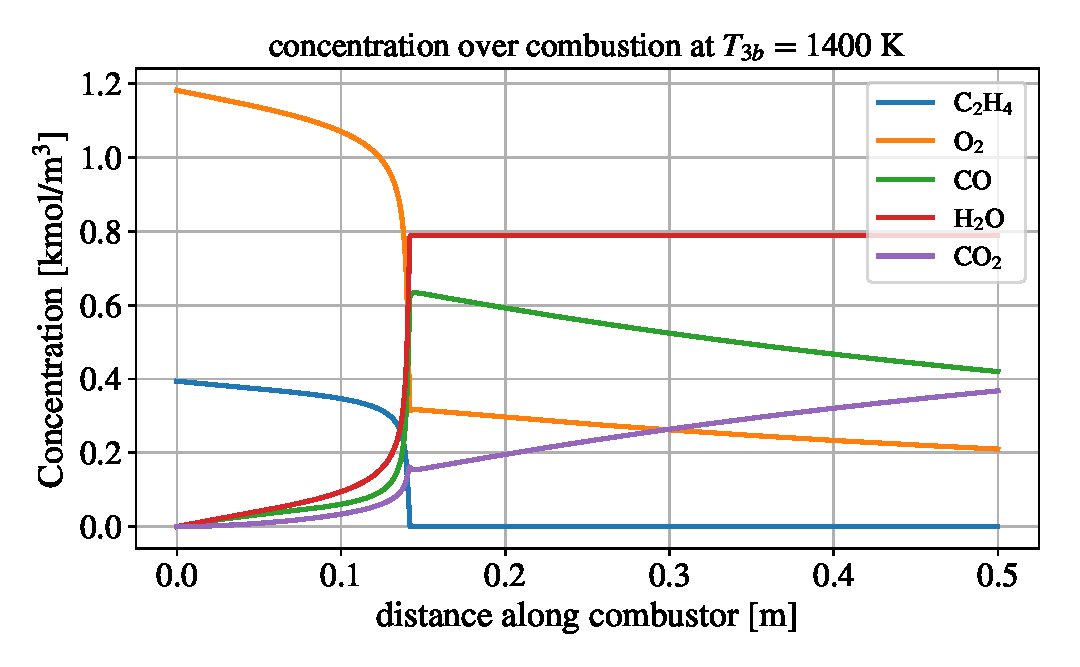
\includegraphics[width=\linewidth]{part_2_img/concentration_1400.pdf}
    %     \caption{Species Concentration}
    %     \label{subfig:concentration_1400}
    % \end{subfigure}
    % \begin{subfigure}[h]{0.49\linewidth}
    %     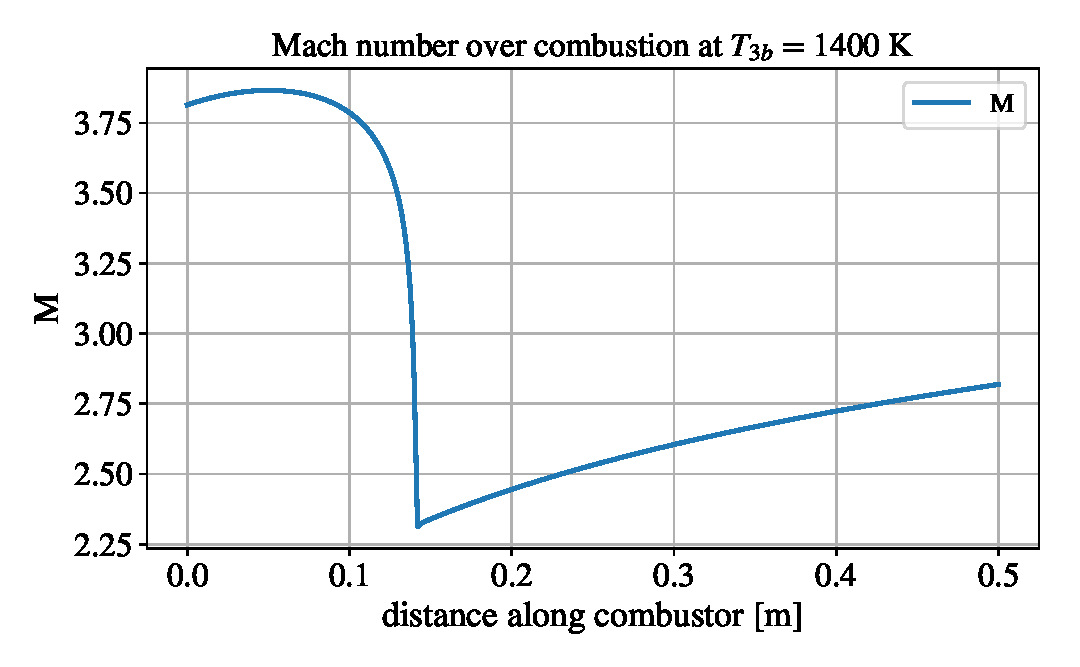
\includegraphics[width=\linewidth]{part_2_img/mach_1400.pdf}
    %     \caption{Mach number}
    %     \label{subfig:mach_1400}
    % \end{subfigure}
    % \begin{subfigure}[h]{0.49\linewidth}
    %     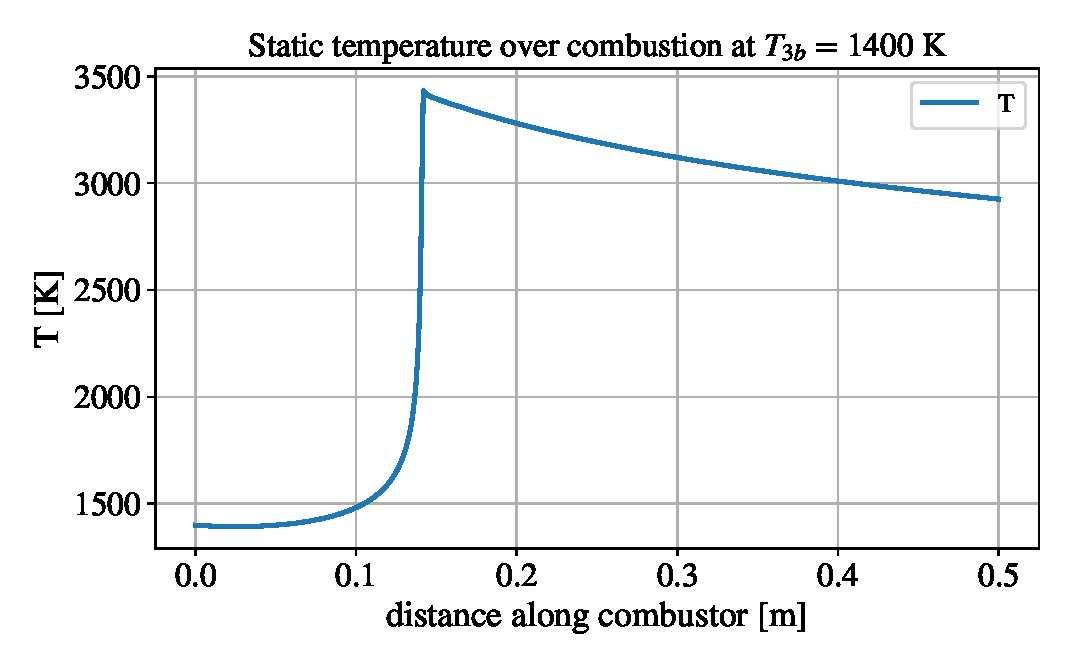
\includegraphics[width=\linewidth]{part_2_img/static_temp_1400.pdf}
    %     \caption{Static temperature}
    %     \label{subfig:temp_1400}
    % \end{subfigure}
    % \begin{subfigure}[h]{0.49\linewidth}
    %     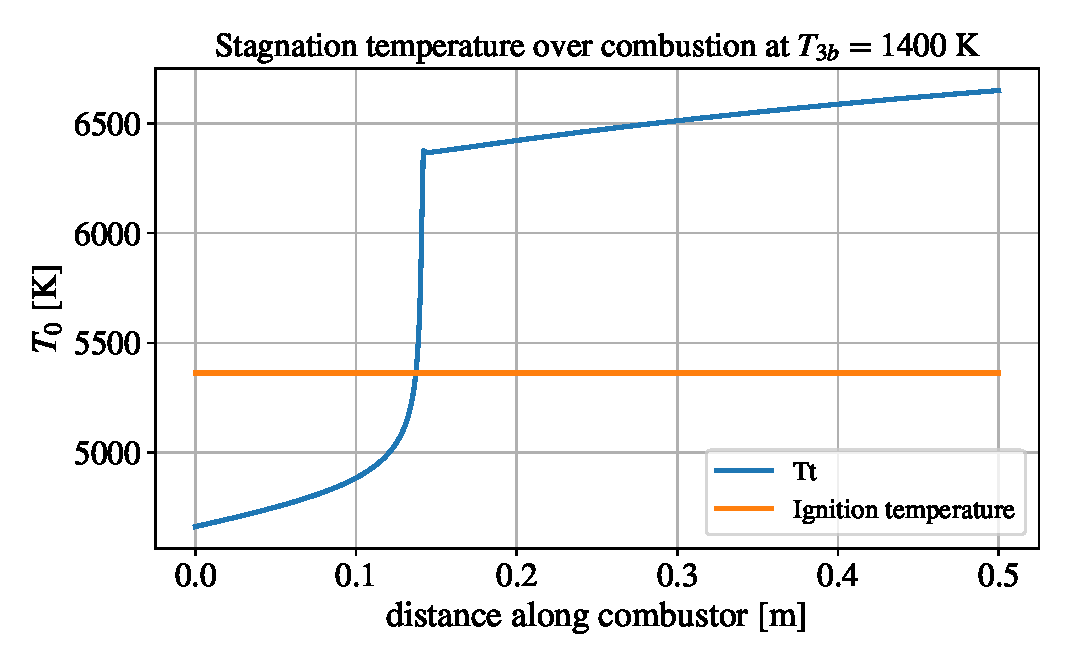
\includegraphics[width=\linewidth]{part_2_img/stag_temp_1400.pdf}
    %     \caption{Stagnation temperature}
    %     \label{subfig:stag_temp_1400}
    % \end{subfigure}
    %  \begin{subfigure}[h]{0.49\linewidth}
    %     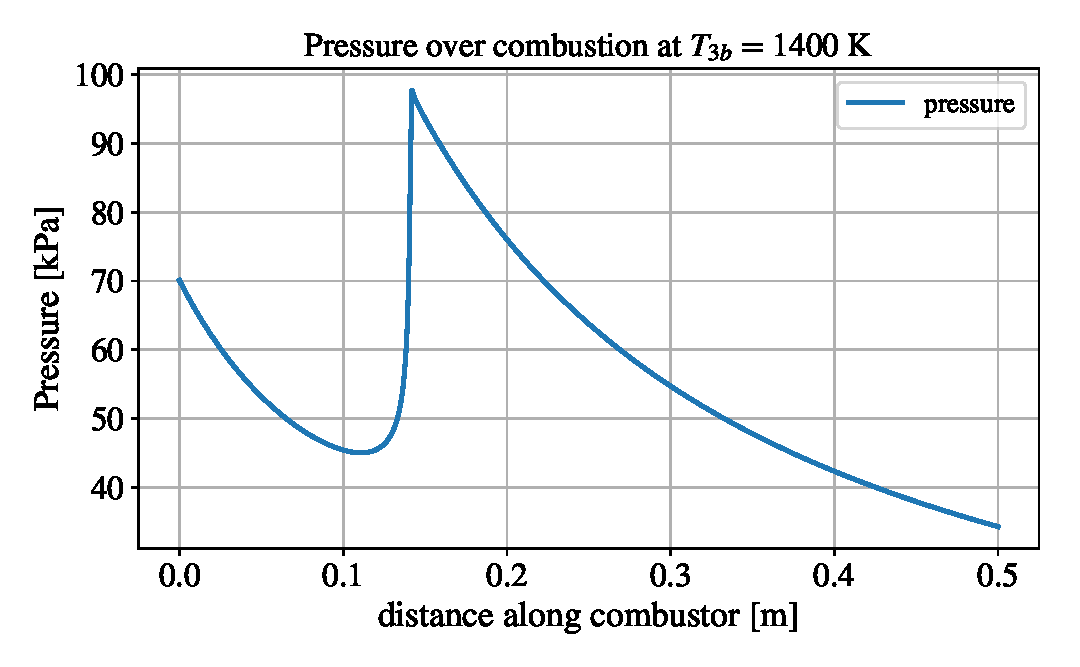
\includegraphics[width=\linewidth]{part_2_img/pressure_1400.pdf}
    %     \caption{Pressure}
    %     \label{subfig:pressure_1400}
    % \end{subfigure}
    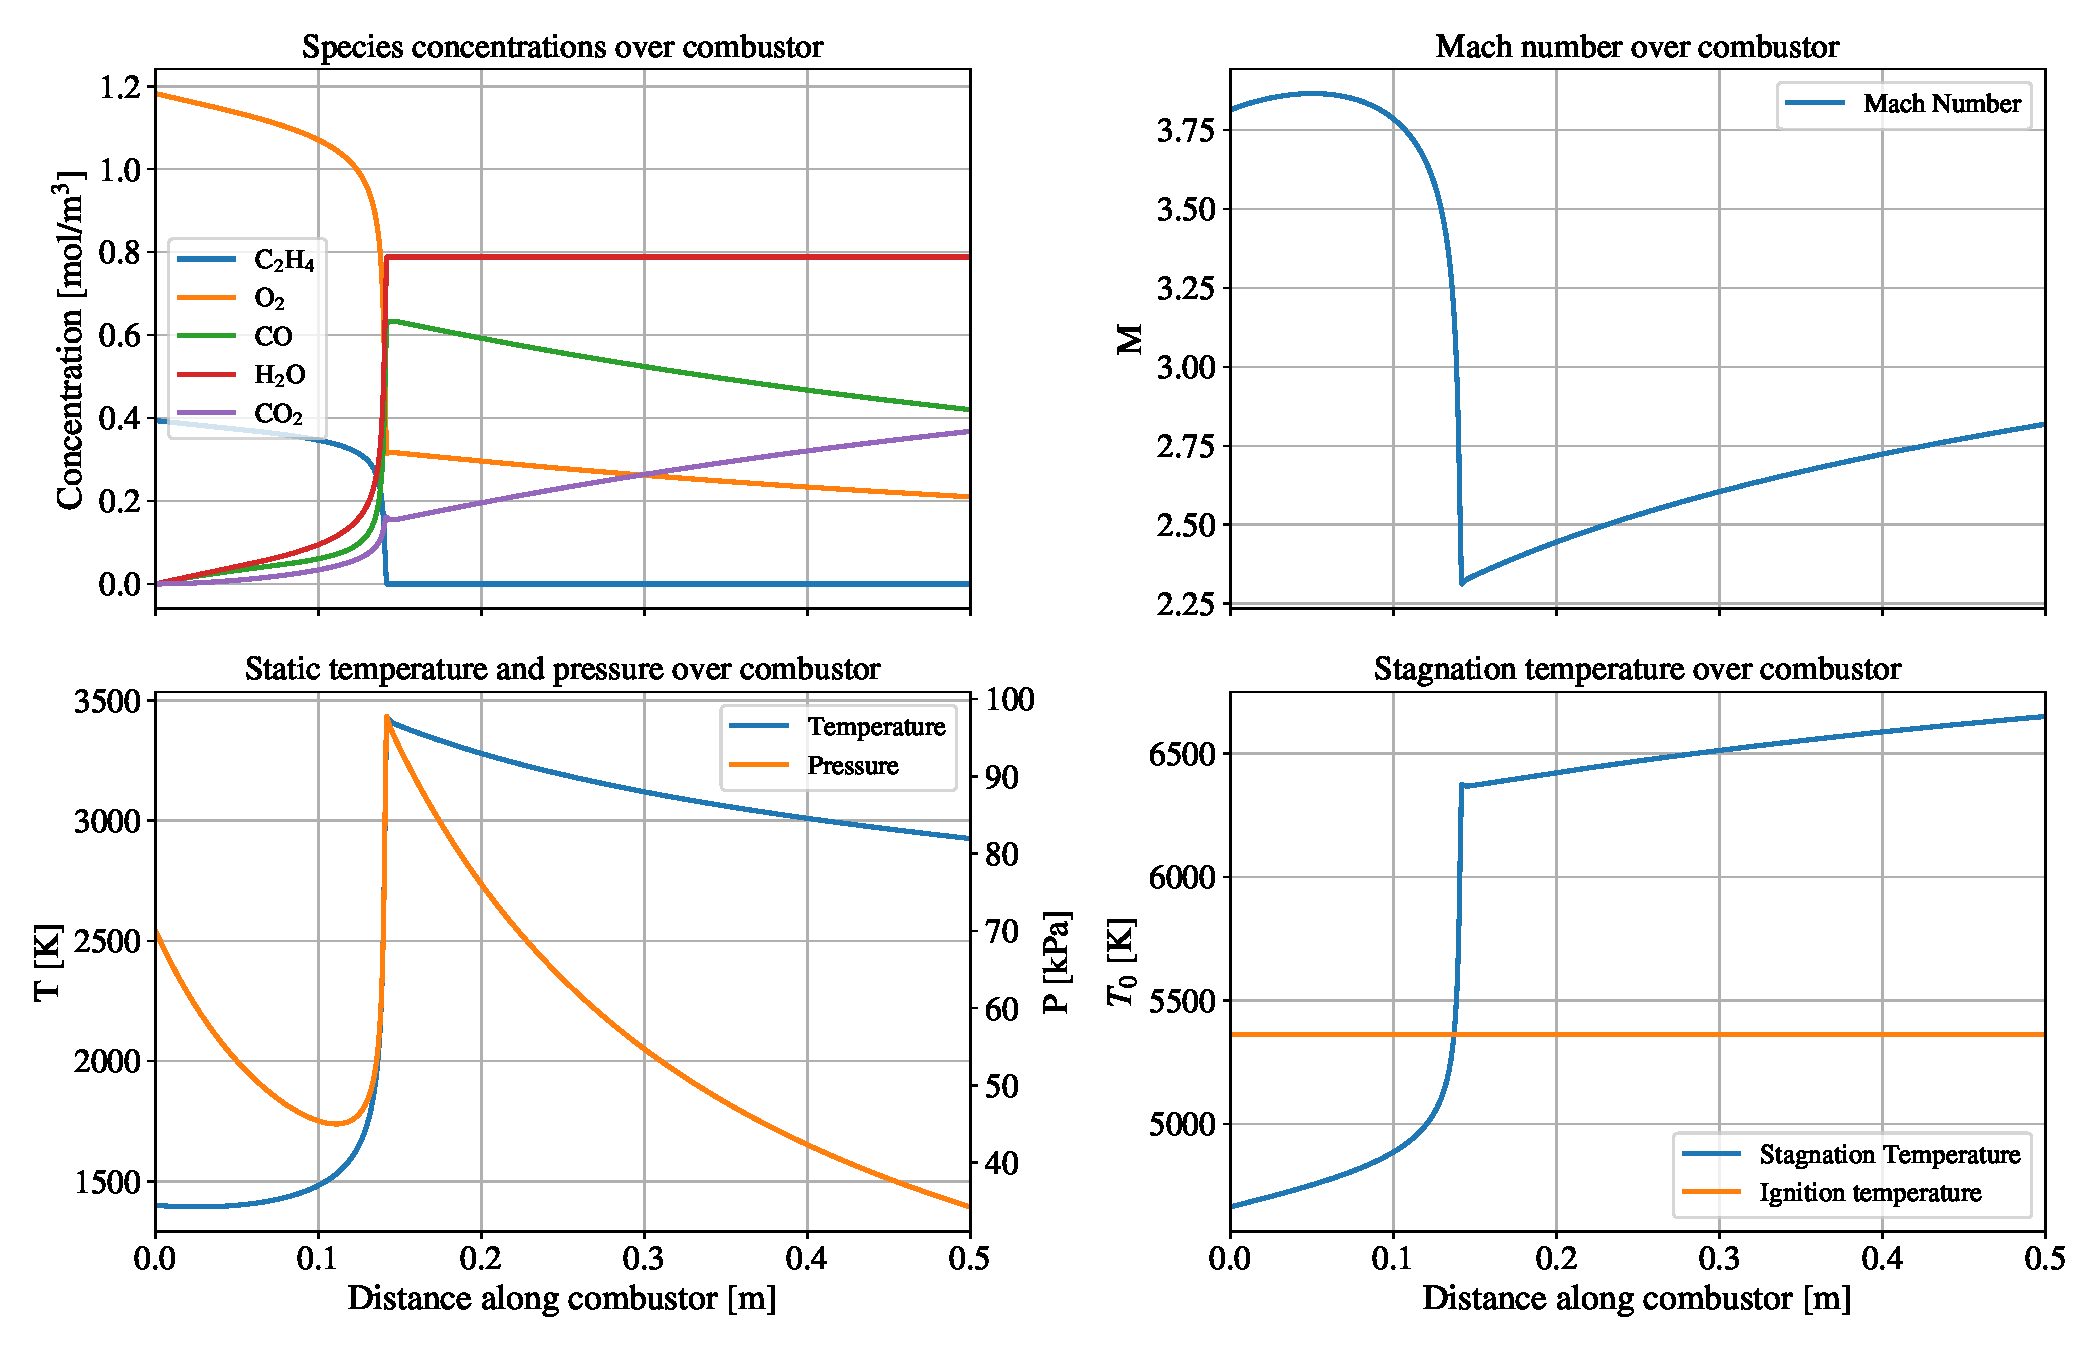
\includegraphics[width=\linewidth]{part_2_img/subfig_1400.pdf}
    \caption{Properties over combustion at 1400~K}
    \label{fig:properties_1400}
\end{widefigure}

\subsection{Nozzle Modelling}
The flow state exiting the nozzle is summarised in Table.~\ref{tab:nozzle_exit_properties}.

\begin{table}[H]
    \centering
    \begin{tabu} spread 0cm {X[-1,l]X[-1,r]}
        \toprule \rowfont[c]{\bfseries} 
         Variable   &         Value         \\
        \midrule
        Mach Number &                  3.82 \\
        Temperature &      \SI{1492.64}{\K} \\
           Pressure &       \SI{2.14}{\kPa} \\
          Exit Area & \SI{2.51}{\m\squared} \\
  Thrust per engine &     \SI{14573.61}{\N} \\
        \bottomrule
    \end{tabu}
    \caption{Nozzle exit properties}
    \label{tab:nozzle_exit_properties}
\end{table}


\subsection{Overall Performance and Discussion}
The overall performance of the scramjet is summarised in Table.~\ref{tab:performance}. 

\begin{table}[H]
    \centering
    \begin{tabu} spread 0cm {X[-1,l]X[-1,r]}
        \toprule \rowfont[c]{\bfseries} 
             Variable     &           Value          \\ 
        \midrule
        Thrust per Engine &        \SI{14573.61}{\N} \\
          Specific Thrust & \SI{468.32}{\N\s\per\kg} \\
         Specific Impulse & \SI{47.74}{\s}\\
                     Drag &        \SI{29031.12}{\N} \\
                Net Force &        \SI{29263.31}{\N} \\
            Thrust Margin & 1.01 \\
        \bottomrule
    \end{tabu}
    \caption{Scramjet Performance}
    \label{tab:performance}
\end{table}

As can be seen, the net thrust is significantly positive, so the four engines provide net thrust to the second stage of the \textsc{Spartan} vehicle. However, the maximum temperature reached within the combustor is approximately 3500~K. This is almost double the current limit of materials. While this is an accelerator engine, the wall temperature likely won't reach this temperature, the wall temperature achieved is likely still going to be above the material limit. To confirm this, further research into whether the wall temperature limit is exceeded is required. 

Another consideration is the performance of the engine at slower speeds, as this is an accelerator engine. The inlet will process the gas differently at different free stream Mach numbers, and the engine may not be able to produce enough thrust to accelerate the vehicle up to Mach 10. Thus inlet and combustion calculations should be performed at different free stream Mach numbers to determine the overall effectiveness of the engine for the given application. 

Some limitations of the model used include:

\begin{itemize}
    \item Assumption of constant \(\gamma_b\), \(R_b\) and \(c_p\),
    \item Assumption of perfectly mixed fuel entering the combustor
    \item Assuming laminar flow, ignoring turbulence within the combustor and nozzle, and ignoring boundary layer effects
    \item Quasi 1 dimensional modelling, ignoring radial flows
    \item No modelling of conductive heat transfer between regions of gas
\end{itemize}

In order to more accurately determine the performance of the engine, computational fluid dynamics techniques are recommended to better account for these limitations.

\section{Conclusion}
The scramjet engine proposed is capable of producing enough thrust to overcome the drag of the \textsc{Spartan} second stage accelerator vehicle based on this analysis. However this analysis also indicated that temperatures within the combustion chamber may be too high for current materials to cope with. Additionally, the performance of the inlet will vary at different speeds, and so the engine may not be able to produce thrust at different speeds. For these reasons, the use of ethylene as the fuel for the scramjet engine isn't ruled out, however further research is required before the feasibility can be definitively determined.

\newpage
\appendix
\section{Plots for other temperatures}\label{app:other_plots}
\begin{widefigure}[20mm]
    \centering
    % \begin{subfigure}[h]{0.49\linewidth}
    %     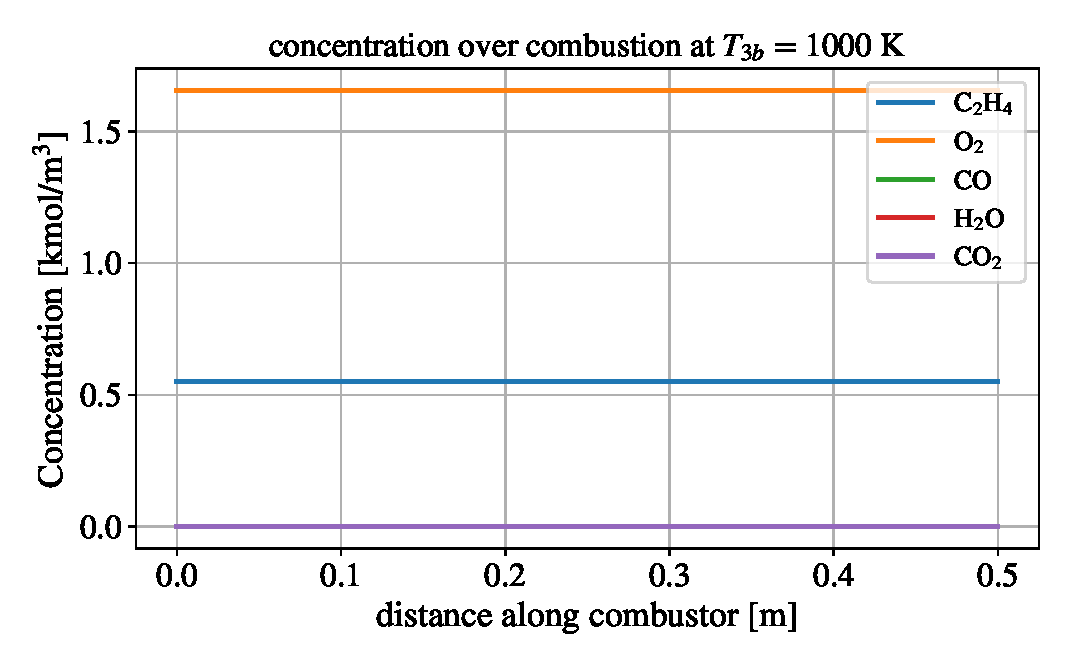
\includegraphics[width=\linewidth]{part_2_img/concentration_1000.pdf}
    %     \caption{Species Concentration}
    %     \label{subfig:concentration_1000}
    % \end{subfigure}
    % \begin{subfigure}[h]{0.49\linewidth}
    %     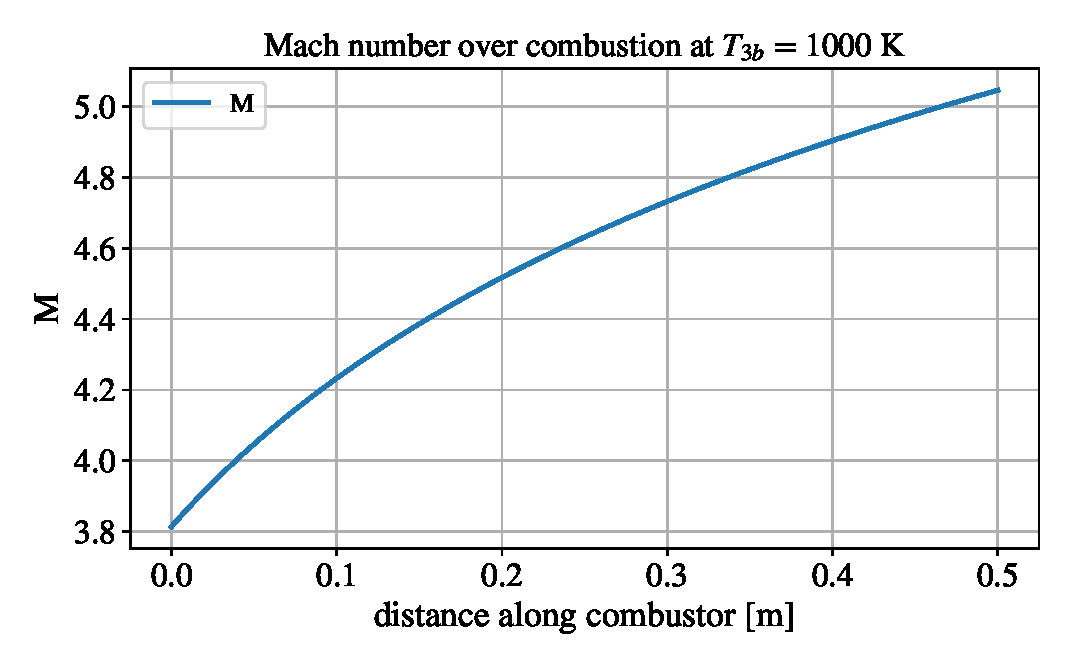
\includegraphics[width=\linewidth]{part_2_img/mach_1000.pdf}
    %     \caption{Mach number}
    %     \label{subfig:mach_1000}
    % \end{subfigure}
    % \begin{subfigure}[h]{0.49\linewidth}
    %     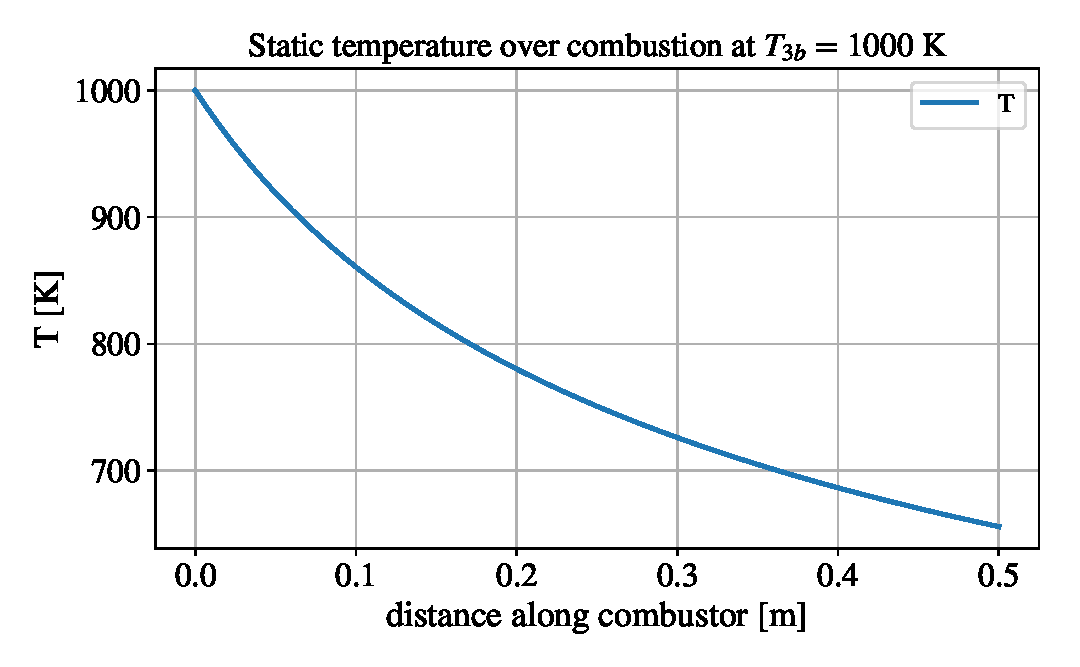
\includegraphics[width=\linewidth]{part_2_img/static_temp_1000.pdf}
    %     \caption{Static temperature}
    %     \label{subfig:temp_1000}
    % \end{subfigure}
    % \begin{subfigure}[h]{0.49\linewidth}
    %     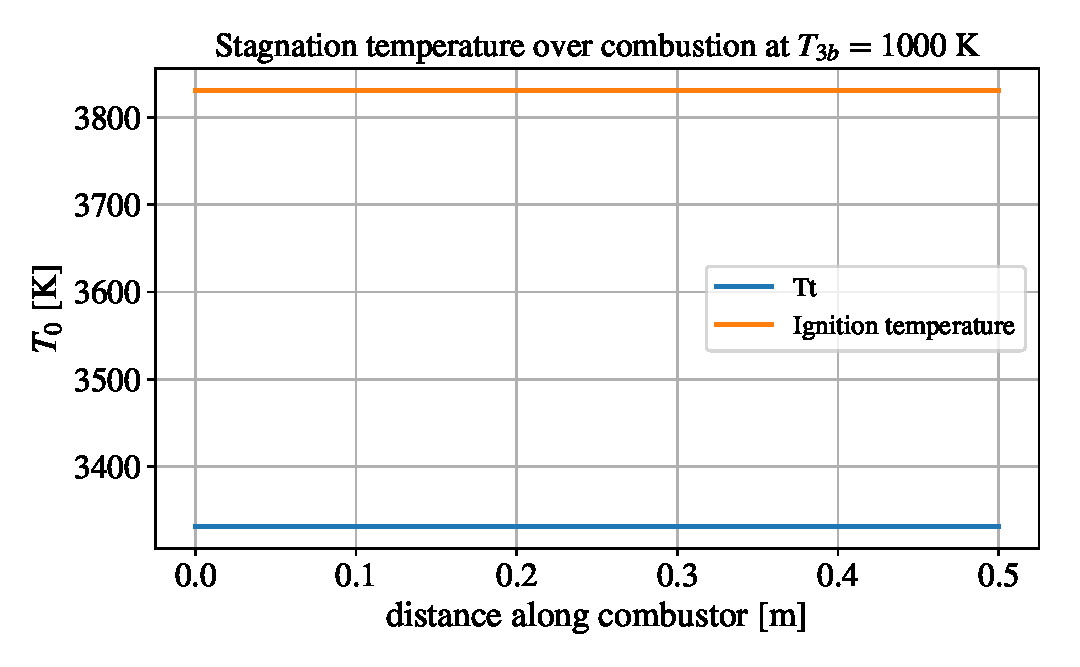
\includegraphics[width=\linewidth]{part_2_img/stag_temp_1000.pdf}
    %     \caption{Stagnation temperature}
    %     \label{subfig:stag_temp_1000}
    % \end{subfigure}
    %  \begin{subfigure}[h]{0.49\linewidth}
    %     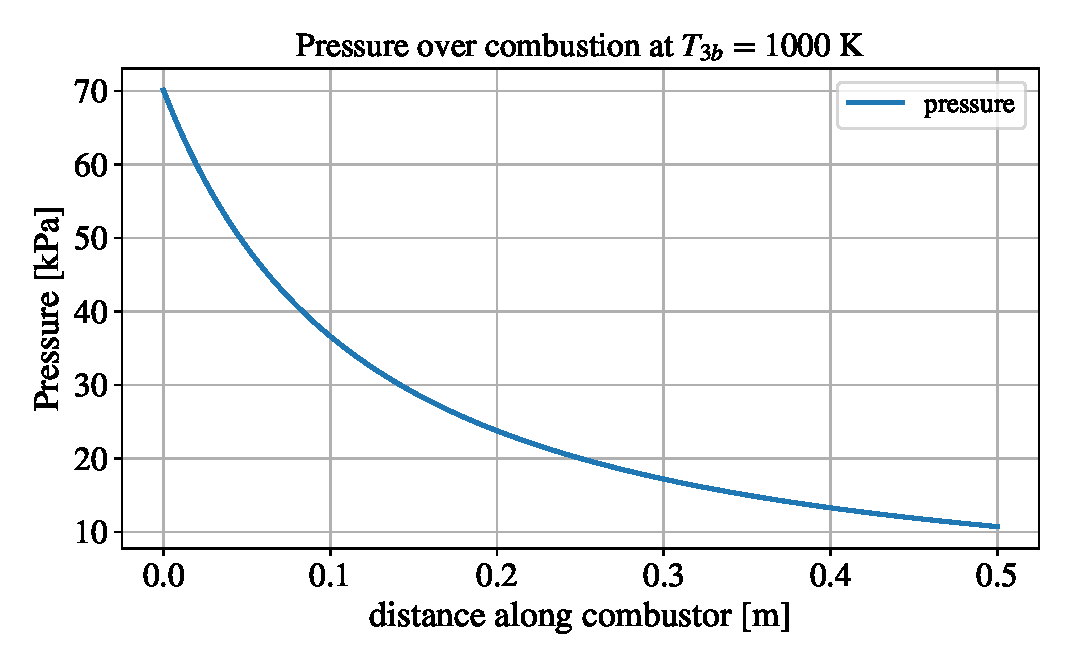
\includegraphics[width=\linewidth]{part_2_img/pressure_1000.pdf}
    %     \caption{Pressure}
    %     \label{subfig:pressure_1000}
    % \end{subfigure}
    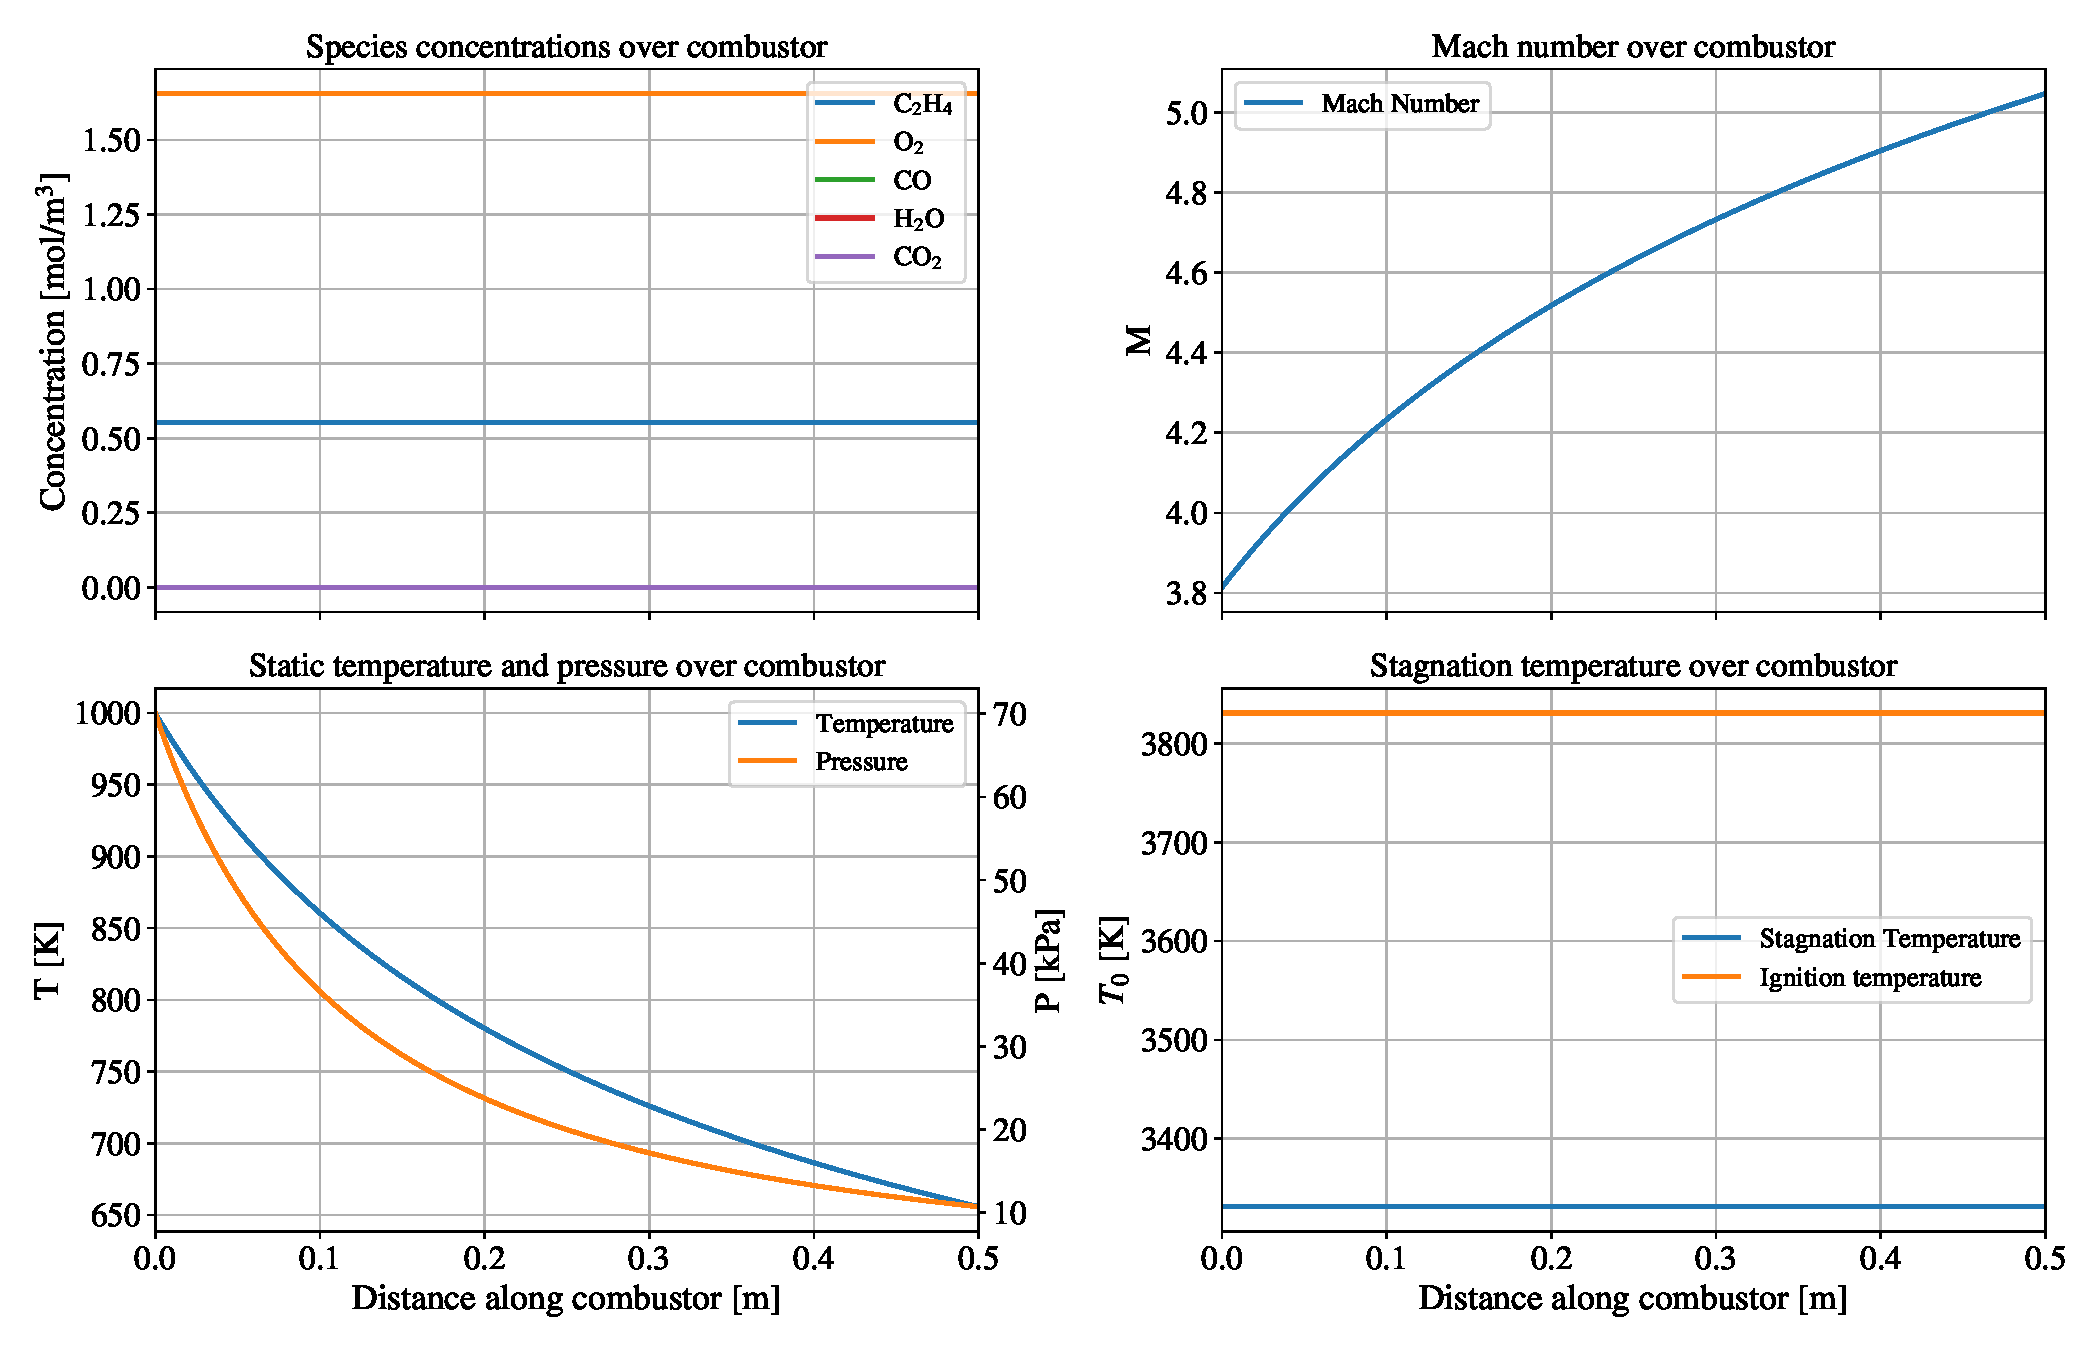
\includegraphics[width=\linewidth]{part_2_img/subfig_1000.pdf}
    \caption{Properties over combustion at \SI{1000}{\K}}
    \label{fig:properties_1000}
\end{widefigure}

\begin{widefigure}[20mm]
    \centering
    % \begin{subfigure}[h]{0.49\linewidth}
    %     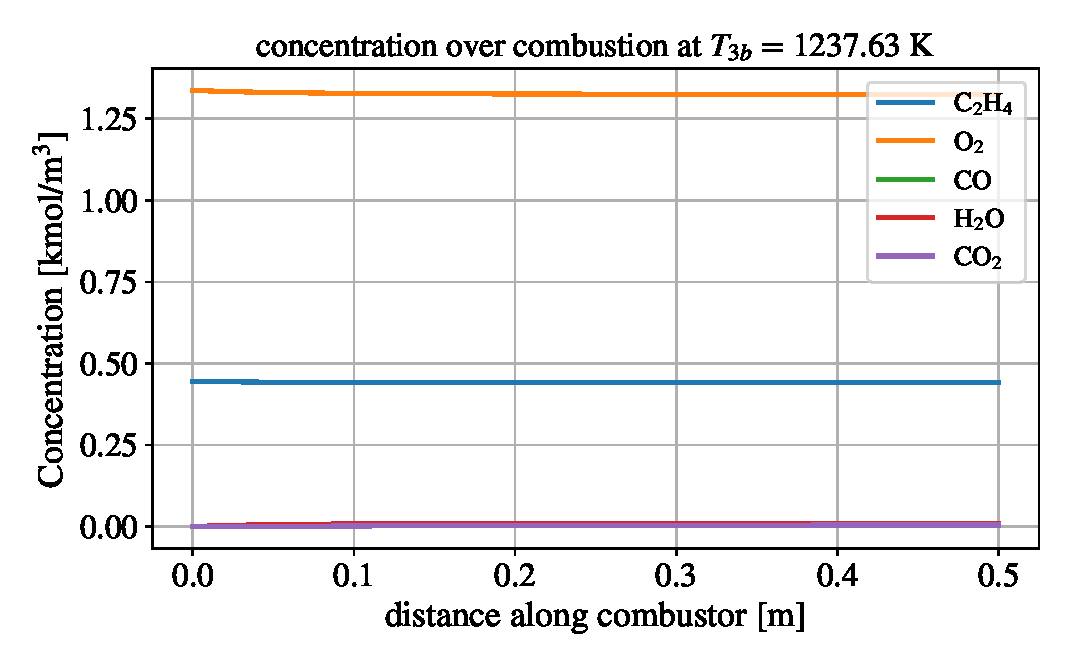
\includegraphics[width=\linewidth]{part_2_img/concentration_1238.pdf}
    %     \caption{Species Concentration}
    %     \label{subfig:concentration_1238}
    % \end{subfigure}
    % \begin{subfigure}[h]{0.49\linewidth}
    %     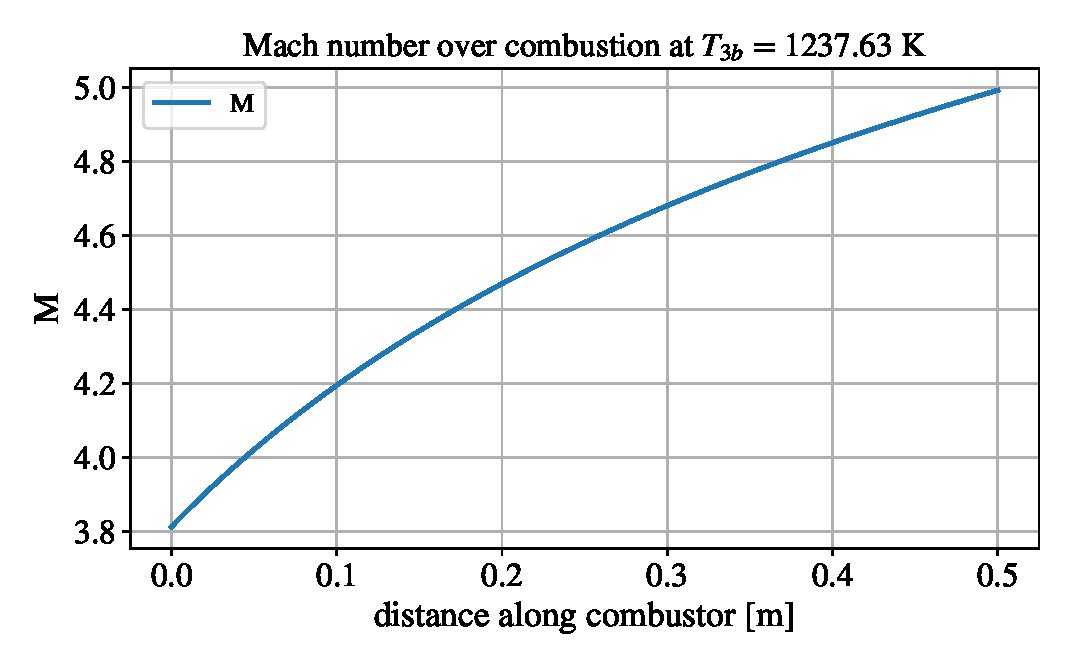
\includegraphics[width=\linewidth]{part_2_img/mach_1238.pdf}
    %     \caption{Mach number}
    %     \label{subfig:mach_1238}
    % \end{subfigure}
    % \begin{subfigure}[h]{0.49\linewidth}
    %     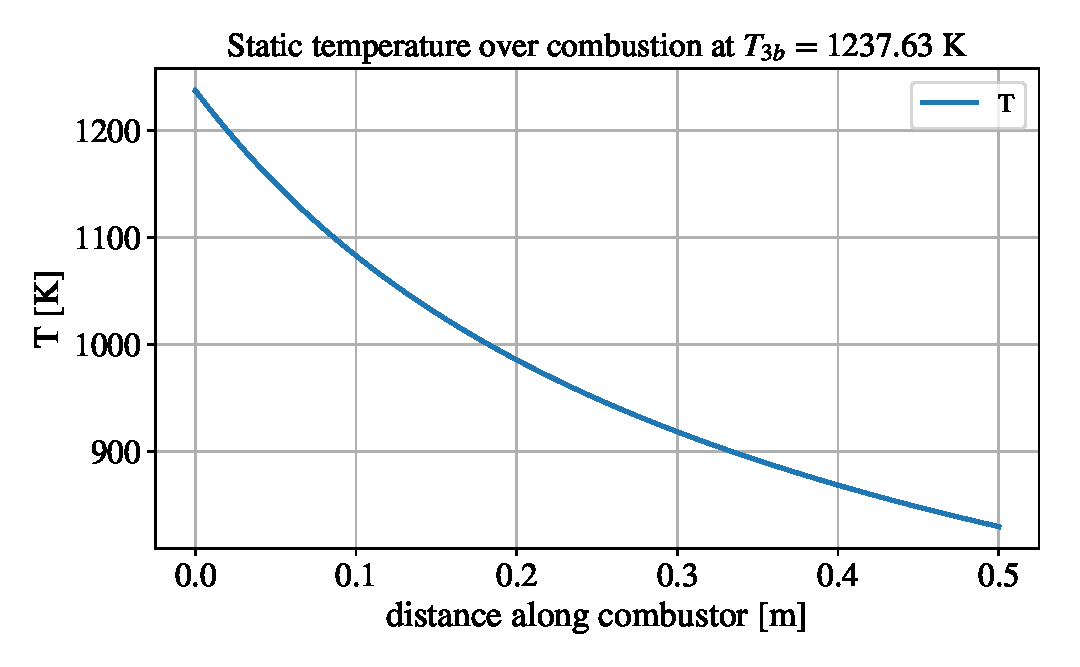
\includegraphics[width=\linewidth]{part_2_img/static_temp_1238.pdf}
    %     \caption{Static temperature}
    %     \label{subfig:temp_1238}
    % \end{subfigure}
    % \begin{subfigure}[h]{0.49\linewidth}
    %     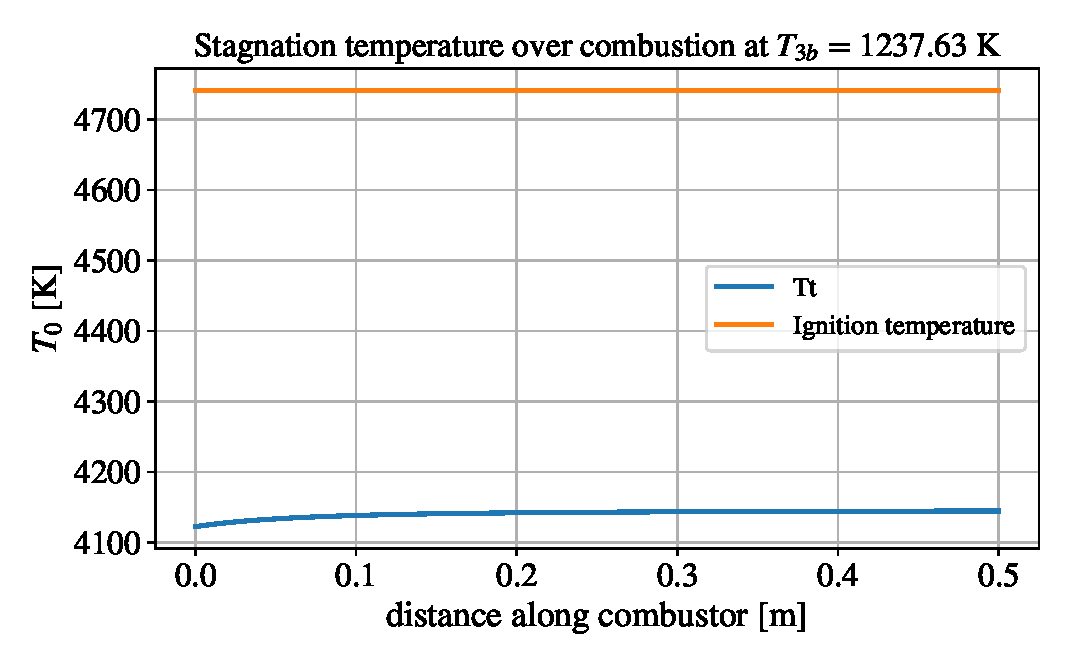
\includegraphics[width=\linewidth]{part_2_img/stag_temp_1238.pdf}
    %     \caption{Stagnation temperature}
    %     \label{subfig:stag_temp_1238}
    % \end{subfigure}
    %  \begin{subfigure}[h]{0.49\linewidth}
    %     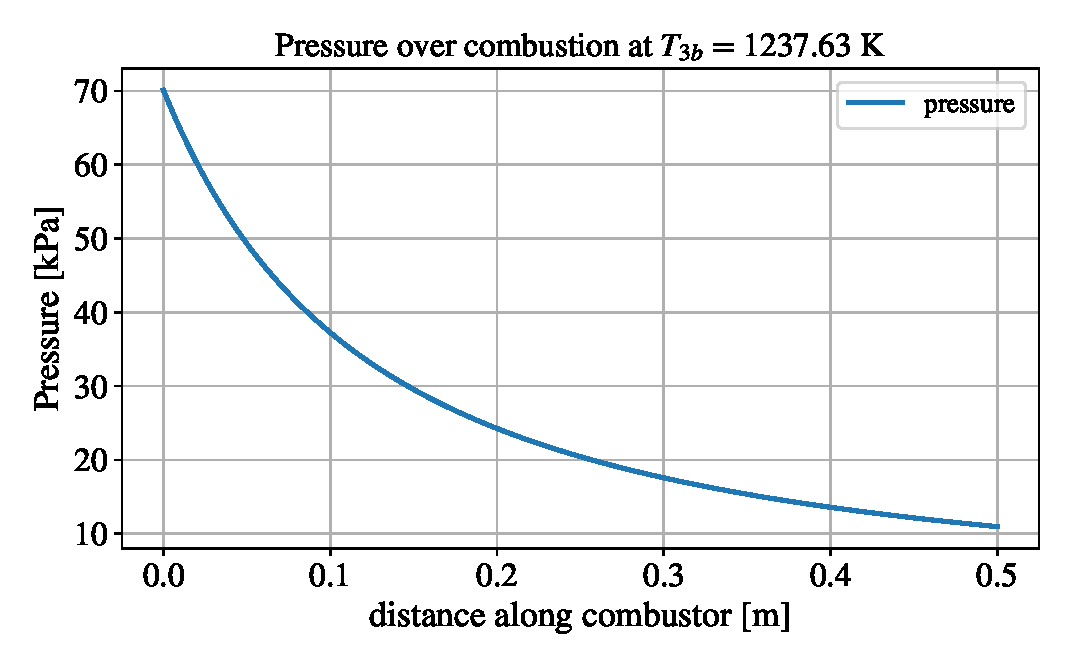
\includegraphics[width=\linewidth]{part_2_img/pressure_1238.pdf}
    %     \caption{Pressure}
    %     \label{subfig:pressure_1238}
    % \end{subfigure}
    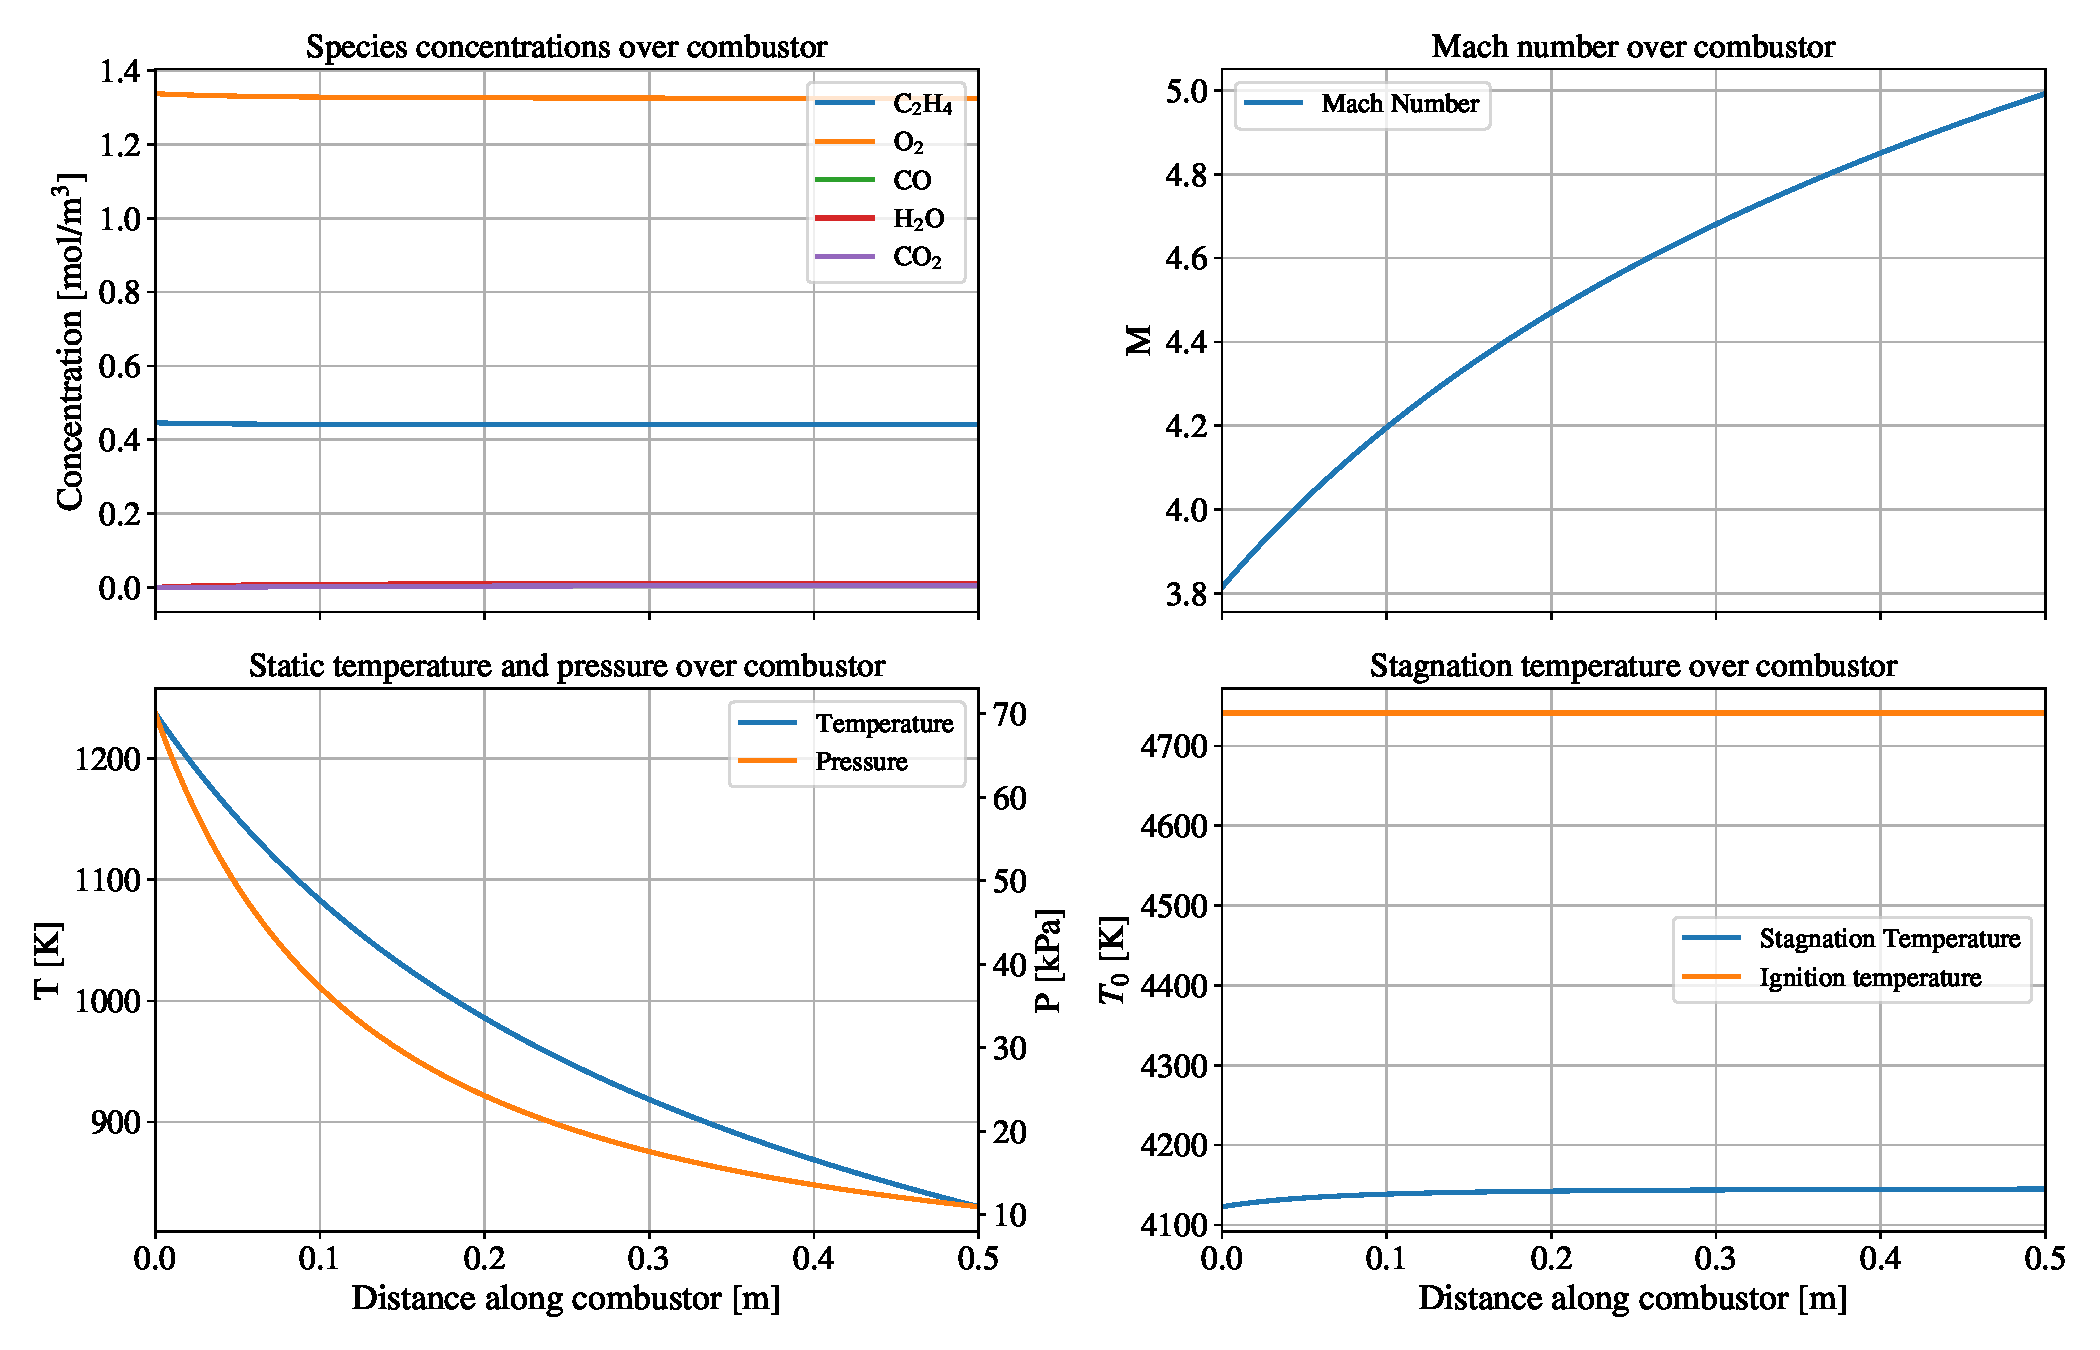
\includegraphics[width=\linewidth]{part_2_img/subfig_1238.pdf}
    \caption{Properties over combustion at \SI{1237.63}{\K}}
    \label{fig:properties_1238}
\end{widefigure}

\newpage
\section{Python Solver}\label{app:code}
\inputminted{python}{code/part2IncludingN2.py}

\end{document}